% ===================================================================
% slides.tex: LCMFreq presentation
% pdflatex + Vietnamese (T5 + babel), 16:9
% ===================================================================
\documentclass[9pt, aspectratio=169]{beamer}

% ---- Encoding & language ------------------------------------------
\usepackage[utf8]{inputenc}
\usepackage[T5]{fontenc}
\usepackage[vietnamese]{babel}
\usefonttheme{serif}
\setbeamertemplate{navigation symbols}{}

% ---- Packages ------------------------------------------------------
\usepackage{xcolor}
\usepackage{amsmath, amssymb}
\usepackage{booktabs}
\usepackage{array}
\usepackage{graphicx}
\usepackage{tikz}
\usetikzlibrary{arrows.meta, positioning, calc, fit, backgrounds}
\usepackage{listings}

% ---- Palette: adapted from psdear.sty ------------------------------
\definecolor{psdearblue}{HTML}{1f4e79}
\definecolor{psdearteal}{HTML}{2a9d8f}
\definecolor{psdearorange}{HTML}{e76f51}
\definecolor{psdeargray}{HTML}{6c757d}
\definecolor{psdearbg}{HTML}{f4f7f9}
\definecolor{psdearnavy}{HTML}{16324f}
\definecolor{psdearsky}{HTML}{d9eef7}
\definecolor{psdeargold}{HTML}{f4a261}
\definecolor{psdeargreen}{HTML}{5c9f72}
\definecolor{psdearink}{HTML}{243746}

% ---- Beamer tone ----------------------------------------------------
\setbeamercolor{normal text}{fg=psdearink,bg=white}
\setbeamercolor{structure}{fg=psdearblue}
\setbeamercolor{frametitle}{fg=psdearnavy,bg=white}
\setbeamerfont{frametitle}{size=\large,series=\bfseries}
\setbeamertemplate{frametitle}{%
  \vspace{0.10em}
  \insertframetitle\strut\par
  \nointerlineskip
  \vspace{0.10em}
  {\color{psdearblue!35}\rule{\linewidth}{0.45pt}}
}
\setbeamertemplate{footline}{%
  \hfill{\color{psdeargray}\scriptsize\insertframenumber/\inserttotalframenumber}\hspace{6pt}\vspace{4pt}
}
\setbeamertemplate{itemize item}{\color{psdearteal}\small$\bullet$}
\setbeamertemplate{itemize subitem}{\color{psdearorange}\scriptsize-{}-}

% ---- Mini table-of-contents shown at the start of every section -----
\setbeamercolor{section in toc}{fg=psdearink}
\setbeamercolor{section in toc shaded}{fg=psdeargray!55}
\setbeamerfont{section in toc}{series=\bfseries}
\AtBeginSection[]{%
  \begin{frame}{Mục lục}
    \tableofcontents[currentsection]
  \end{frame}
}

% ---- Compact boxes: quieter than full beamer blocks ----------------
\newenvironment{quietblock}[1]{%
  \begin{beamercolorbox}[wd=\linewidth,sep=5pt,rounded=true]{block body}
  {\color{psdearblue}\bfseries #1}\par\vspace{2pt}\footnotesize
}{%
  \end{beamercolorbox}
}
\setbeamercolor{block body}{bg=psdearbg,fg=psdearink}

\newcommand{\key}[1]{\textcolor{psdearblue}{\textbf{#1}}}
\newcommand{\orange}[1]{\textcolor{psdearorange}{#1}}
\newcommand{\teal}[1]{\textcolor{psdearteal}{#1}}

% ---- Listings -------------------------------------------------------
\lstdefinelanguage{JuliaLite}{
  morekeywords={function,end,for,in,if,else,elseif,return,do,continue,let,begin},
  sensitive=true,
  morecomment=[l]\#,
  morestring=[b]"
}
\lstset{
  language=JuliaLite,
  basicstyle=\ttfamily\scriptsize,
  keywordstyle=\color{psdearblue}\bfseries,
  commentstyle=\color{psdeargray},
  stringstyle=\color{psdearteal},
  columns=fullflexible,
  keepspaces=true,
  showstringspaces=false,
  frame=single,
  rulecolor=\color{psdearblue!35},
  backgroundcolor=\color{psdearbg},
  xleftmargin=0.5em,
  xrightmargin=0.5em,
  aboveskip=3pt,
  belowskip=3pt
}

% ---- TikZ styles ----------------------------------------------------
\tikzset{
  tx/.style={draw=psdearblue!65, fill=psdearsky!45, rounded corners=2pt,
             minimum width=3.2cm, minimum height=0.58cm, align=center, font=\scriptsize},
  bucket/.style={draw=psdeargreen!70!black, fill=psdeargreen!10,
                 rounded corners=2pt, minimum width=2.35cm, minimum height=0.82cm,
                 align=center, font=\scriptsize},
  arrow/.style={-{Latex[length=1.8mm,width=1.2mm]}, line width=0.65pt},
  nodebox/.style={draw=psdearblue!70, fill=psdearsky!35, rounded corners=2pt,
                  align=center, inner sep=4pt, font=\scriptsize}
}

\title{LCMFreq}
\subtitle{Khai thác tập phổ biến bằng Backtracking, OccurrenceDeliver và Hypercube}
\author{Nhóm 01, CSC14004}
\date{HCMUS, 2025--2026}

\begin{document}

% -------------------------------------------------------------------
\begin{frame}[plain]
  \begin{center}
    {\small ĐẠI HỌC QUỐC GIA TP. HỒ CHÍ MINH}\\
    {\small TRƯỜNG ĐẠI HỌC KHOA HỌC TỰ NHIÊN}\\
    {\small KHOA CÔNG NGHỆ THÔNG TIN}\\[0.35cm]
    {\color{psdearblue}\rule{0.62\linewidth}{0.6pt}}\\[0.3cm]
    {\Large\bfseries\color{psdearnavy} LCMFreq}\\[0.18cm]
    {\large Khai thác tập phổ biến bằng Backtracking, OccurrenceDeliver và Hypercube}\\[0.3cm]
    {\color{psdearblue}\rule{0.62\linewidth}{0.6pt}}
  \end{center}

  \vspace{0.35cm}
  \begin{columns}[T,onlytextwidth]
    \begin{column}{0.56\textwidth}
      \small
      \textbf{Sinh viên thực hiện}
      \vspace{0.1cm}

      \begin{tabular}{@{}c l c@{}}
        \toprule
        STT & Họ và tên & MSSV \\
        \midrule
        1 & Phạm Phú Hòa (nhóm trưởng) & 23122030 \\
        2 & Huỳnh Trung Kiệt & 23122039 \\
        3 & Đào Sỹ Duy Minh & 23122041 \\
        4 & Trần Chí Nguyên & 23122044 \\
        5 & Nguyễn Lâm Phú Quý & 23122048 \\
        \bottomrule
      \end{tabular}
    \end{column}
    \begin{column}{0.40\textwidth}
      \small
      \textbf{Giảng viên hướng dẫn}\\[0.1cm]
      GS.TS. Lê Hoài Bắc\\
      ThS. Nguyễn Thị Thu Hằng\\
      ThS. Nguyễn Ngọc Đức\\
      ThS. Lê Nhựt Nam\\[0.3cm]
      \textbf{Môn học}\\
      CSC14004, Khai thác dữ liệu và ứng dụng
    \end{column}
  \end{columns}

  \vfill
  {\scriptsize\color{psdeargray}HCMUS, học kỳ 2, năm học 2025--2026}
\end{frame}

% -------------------------------------------------------------------
\begin{frame}{Nội dung trình bày}
  \tableofcontents
\end{frame}

% ===================================================================
\section{Đặt vấn đề}
% ===================================================================
\begin{frame}{Định nghĩa hình thức (Uno, Kiyomi, Arimura, 2004, Mục 2)}
  \begin{quietblock}{Transaction database và itemset}
    Gọi $\mathcal I=\{1,\ldots,n\}$ là tập item. Một transaction database
    trên $\mathcal I$ là tập $\mathcal D=\{T_1,\ldots,T_m\}$, mỗi $T_i$ là
    một tập con của $\mathcal I$, gọi là một giao dịch. Một tập con
    $P\subseteq\mathcal I$ được gọi là một itemset.
  \end{quietblock}

  \vspace{0.2cm}
  \begin{quietblock}{Denotation và frequency}
    Với itemset $P$, một giao dịch chứa $P$ được gọi là một occurrence của
    $P$. Tập tất cả occurrence của $P$ được gọi là denotation của $P$, ký
    hiệu $\mathcal T(P)$. Số lượng $|\mathcal T(P)|$ gọi là frequency của
    $P$ (trong nhiều tài liệu khác gọi là support), ký hiệu
    $\mathrm{sup}(P)$. Với ngưỡng tối thiểu $\sigma$ cho trước, itemset $P$
    là \key{frequent} nếu $\mathrm{sup}(P)\geq\sigma$.
  \end{quietblock}

  \vspace{0.2cm}
  \begin{quietblock}{Hai tính chất nền tảng}
    Với hai itemset $P,Q$ bất kỳ: $\mathcal T(P\cup Q)=\mathcal T(P)\cap
    \mathcal T(Q)$. Và nếu $P\subseteq Q$ thì $\mathcal T(Q)\subseteq
    \mathcal T(P)$, do đó $\mathrm{sup}(Q)\leq\mathrm{sup}(P)$. Bài toán
    Frequent Itemset Mining yêu cầu tìm toàn bộ itemset frequent của một
    database cho trước, không bỏ sót.
  \end{quietblock}
\end{frame}

% -------------------------------------------------------------------
\begin{frame}{Tính đơn điệu và thứ tự sinh itemset}
  \begin{quietblock}{Tính chất đơn điệu (monotone property)}
    Từ $P\subseteq Q\Rightarrow\mathcal T(Q)\subseteq\mathcal T(P)$, suy ra
    nếu $P$ không frequent thì mọi superset của $P$ cũng không frequent.
    Nhờ tính chất này, mọi frequent itemset đều có thể được xây dựng từ tập
    rỗng bằng cách thêm item lần lượt, mà không cần đi qua một itemset
    không frequent nào ở giữa.
  \end{quietblock}

  \vspace{0.15cm}
  \begin{quietblock}{tail(P) và quy tắc sinh không trùng}
    Gọi $\mathrm{tail}(P)$ là item có chỉ số lớn nhất trong $P$. Khung
    backtracking chỉ thêm vào $P$ những item $e>\mathrm{tail}(P)$. Nếu
    không có quy tắc này, một itemset như $\{A,C,D\}$ có thể sinh ra từ
    nhiều thứ tự thêm khác nhau và bị tính trùng. Với quy tắc trên, mỗi
    itemset chỉ có đúng một đường sinh duy nhất.
  \end{quietblock}

  \vspace{0.15cm}
  \centering
  \resizebox{0.56\linewidth}{!}{%
  \begin{tikzpicture}[font=\scriptsize]
    \node[nodebox, minimum width=2.2cm] (root) at (0,0) {$\emptyset$};

    \node[nodebox, minimum width=1.9cm] (A) at (-3.2,-1.35) {$A$};
    \node[nodebox, minimum width=1.9cm] (C) at (0,-1.35) {$C$};
    \node[nodebox, minimum width=1.9cm] (D) at (3.2,-1.35) {$D$};

    \node[nodebox, minimum width=1.9cm] (AC) at (-4.1,-2.7) {$A,C$};
    \node[nodebox, minimum width=1.9cm] (AD) at (-2.3,-2.7) {$A,D$};
    \node[nodebox, minimum width=1.9cm] (CD) at (0.9,-2.7) {$C,D$};

    \node[nodebox, minimum width=2.2cm, fill=psdeargreen!10, draw=psdeargreen!70!black]
      (ACD) at (-4.1,-4.05) {$A,C,D$};

    \draw[arrow,draw=psdearblue] (root) -- node[left]{$A$} (A);
    \draw[arrow,draw=psdearblue] (root) -- node[right]{$C$} (C);
    \draw[arrow,draw=psdearblue] (root) -- node[right]{$D$} (D);
    \draw[arrow,draw=psdearblue] (A) -- node[left]{$C$} (AC);
    \draw[arrow,draw=psdearblue] (A) -- node[right]{$D$} (AD);
    \draw[arrow,draw=psdearblue] (C) -- node[right]{$D$} (CD);
    \draw[arrow,draw=psdearteal] (AC) -- node[left]{$D$} (ACD);

    \node[align=center, text=psdeargray] at (1.1,-4.0)
      {Chỉ đi xuống item lớn hơn $\mathrm{tail}(P)$, nên không sinh lại cùng itemset.};
  \end{tikzpicture}}
\end{frame}

% ===================================================================
\section{Khung Backtracking}
% ===================================================================
\begin{frame}{Hai nhóm thuật toán cho Frequent Itemset Mining}
  \begin{quietblock}{Nhóm Apriori (level by level)}
    Gọi $\mathcal D_k$ là tập frequent itemset kích thước $k$. Apriori tính
    $\mathcal D_k$ từ $\mathcal D_{k-1}$ theo thứ tự $k$ tăng dần, bằng cách
    thêm mỗi item vào từng itemset của $\mathcal D_{k-1}$ rồi giữ lại các
    itemset frequent. Toàn bộ $\mathcal D_{k-1}$ phải được lưu trong bộ nhớ
    để sinh $\mathcal D_k$.
  \end{quietblock}

  \vspace{0.15cm}
  \begin{quietblock}{Nhóm Backtracking}
    Mỗi lượt đệ quy nhận một frequent itemset $P$ (nghiệm hiện tại), thêm
    từng item vào $P$, rồi đệ quy tiếp với các itemset con frequent. Chỉ
    nghiệm hiện tại được giữ trong bộ nhớ, không cần lưu lại các itemset đã
    sinh trước đó.
  \end{quietblock}

  \vspace{0.2cm}
  \small
  Theo Uno et al. (2004): \textit{``Apriori algorithms use much memory for
  storing $\mathcal D_k$, while backtracking algorithms use less memory
  since they keep only the current solution... However, apriori algorithms
  have advantages for the frequency counting.''} Đây chính là động cơ của
  LCMFreq: chọn khung backtracking để tiết kiệm bộ nhớ, đồng thời khắc phục
  điểm yếu của backtracking trong việc đếm support, bằng hai kỹ thuật trình
  bày ở các phần sau.
\end{frame}

% -------------------------------------------------------------------
\begin{frame}[fragile]{Khung thuật toán BackTracking}
  \begin{columns}[T,onlytextwidth]
    \begin{column}{0.46\textwidth}
\begin{lstlisting}
BackTracking(P: nghiem hien tai):
    output P
    for e in I, e > tail(P):
        if P union {e} la frequent:
            BackTracking(P union {e})
\end{lstlisting}
    \end{column}
    \begin{column}{0.5\textwidth}
      \small
      Mỗi lượt gọi xuất ra itemset $P$ hiện tại, rồi thử thêm từng item $e$
      lớn hơn $\mathrm{tail}(P)$. Nếu $P\cup\{e\}$ frequent thì gọi đệ quy
      tiếp với $P\cup\{e\}$.

      \vspace{0.15cm}
      Khung này tạo ra một cây tìm kiếm: mỗi node là một lượt gọi, mỗi cạnh
      ứng với việc thêm một item. LCMFreq giữ đúng khung này, và chỉ thay
      đổi cách thực hiện hai việc bên trong: đếm support nhanh hơn (phần
      OccurrenceDeliver), và xuất kết quả theo lô (phần HypercubeDecomposition).
    \end{column}
  \end{columns}
\end{frame}

% -------------------------------------------------------------------
\begin{frame}{Ba kỹ thuật của LCMFreq trên khung Backtracking}
  \begin{columns}[T,onlytextwidth]
    \begin{column}{0.32\textwidth}
      \begin{quietblock}{1. Backtracking}
        Mỗi node trong cây tìm kiếm là một prefix $P$. Chỉ thêm item
        $e>\mathrm{tail}(P)$, để mỗi itemset có đúng một đường sinh.
      \end{quietblock}
    \end{column}
    \begin{column}{0.32\textwidth}
      \begin{quietblock}{2. OccurrenceDeliver}
        Tại node $P$, duyệt các giao dịch trong $\mathcal T(P)$ một lần,
        rồi đưa từng giao dịch vào bucket của mọi item nó chứa.
      \end{quietblock}
    \end{column}
    \begin{column}{0.32\textwidth}
      \begin{quietblock}{3. Hypercube}
        Nếu thêm $e$ không làm giảm denotation, mọi tổ hợp chứa các item
        như vậy đều cùng support, và có thể xuất ra ngay một lượt.
      \end{quietblock}
    \end{column}
  \end{columns}

  \vspace{0.45cm}
  \centering
  \resizebox{0.96\linewidth}{!}{%
  \begin{tikzpicture}[font=\footnotesize]
    \node[nodebox, minimum width=2.6cm] (p) at (0,0) {$P$};
    \node[nodebox, minimum width=2.8cm] (bucket) at (4,0) {Buckets\\$\mathrm{Bucket}[e]$};
    \node[nodebox, minimum width=3.3cm] (h) at (8.5,0) {$H(P)$\\item miễn phí};
    \node[nodebox, minimum width=3.2cm] (out) at (12.5,0) {Xuất\\$P\cup Q,\ Q\subseteq S'$};
    \draw[arrow,draw=psdearblue] (p) -- node[above]{deliver} (bucket);
    \draw[arrow,draw=psdearteal] (bucket) -- node[above]{cùng support} (h);
    \draw[arrow,draw=psdearorange] (h) -- node[above]{xuất theo lô} (out);
  \end{tikzpicture}}

  \vspace{0.15cm}
  {\scriptsize\color{psdeargray}\centering Deliver để biết support của mọi
  candidate cùng lúc, sau đó lọc ra các item miễn phí (không giảm support),
  xuất tất cả tổ hợp của các item miễn phí đó trong một lần, rồi mới đệ quy
  tiếp với các item còn lại.\par}
\end{frame}

% ===================================================================
\section{Đếm support hiệu quả}
% ===================================================================
\begin{frame}{Down project: cách tổng quát để tính denotation}
  \begin{quietblock}{Định nghĩa down project}
    Với itemset $P=P_1\cup P_2$, ta có $\mathcal T(P)=\mathcal T(P_1)\cap
    \mathcal T(P_2)$. Nếu các item trong $\mathcal T(P_1)$ và $\mathcal
    T(P_2)$ đã được sắp theo chỉ số, phép giao này tính được trong
    $O(|\mathcal T(P_1)|+|\mathcal T(P_2)|)$, bằng cách đi hai con trỏ song
    song qua hai danh sách đã sort.
  \end{quietblock}

  \vspace{0.2cm}
  \begin{quietblock}{Vấn đề khi áp dụng cho backtracking}
    Down project hiệu quả nếu chọn được cặp $P_1,P_2$ tốt, điều Apriori có
    thể làm. Nhưng backtracking luôn thêm đúng một item mỗi lượt, nên cặp
    tách duy nhất có thể dùng là $P_1=P$, $P_2=\{e\}$. Với $k$ candidate
    $e>\mathrm{tail}(P)$, chi phí tính theo down project là:
    \[
      O\!\left(\sum_{e>\mathrm{tail}(P)} \bigl(|\mathcal T(P)|+|\mathcal
      T(\{e\})|\bigr)\right).
    \]
    Số hạng $|\mathcal T(P)|$ bị cộng lặp lại cho từng candidate $e$, dù
    $\mathcal T(P)$ không đổi giữa các lần đó.
  \end{quietblock}
\end{frame}

% -------------------------------------------------------------------
\begin{frame}{Vì sao OccurrenceDeliver nhanh hơn: ví dụ đếm bước}
  \small
  Xét node $P=\{A\}$, với $\mathcal T(P)=\{t_1,t_3,t_5\}$ là ba giao dịch
  đang chứa $A$, trong đó $t_1=\{A,B,C\}$, $t_3=\{A,C,D\}$, $t_5=\{A,B,D\}$.
  Giả sử $\mathcal T(B),\mathcal T(C),\mathcal T(D)$ đã có sẵn từ lượt quét
  database lúc đầu, với độ dài lần lượt là 5, 4, 3.
  \begin{columns}[T,onlytextwidth]
    \begin{column}{0.48\textwidth}
      \begin{quietblock}{Down project: tính riêng từng candidate}
        Theo công thức ở slide trước:
        \begin{itemize}
          \item $\mathcal T(P)\cap\mathcal T(B)$: $3+5=8$ bước
          \item $\mathcal T(P)\cap\mathcal T(C)$: $3+4=7$ bước
          \item $\mathcal T(P)\cap\mathcal T(D)$: $3+3=6$ bước
        \end{itemize}
        Tổng \textbf{21 bước}. $\mathcal T(P)$ (3 phần tử) bị đọc lại
        \textbf{3 lần}, một lần cho mỗi candidate.
      \end{quietblock}
    \end{column}

    \begin{column}{0.48\textwidth}
      \begin{quietblock}{OccurrenceDeliver: tính một lần cho cả ba}
        Duyệt ba giao dịch đúng một lần, mỗi giao dịch tốn bằng số item nó
        có ngoài $A$:
        \begin{itemize}
          \item $t_1$ có $B,C$: 2 bước
          \item $t_3$ có $C,D$: 2 bước
          \item $t_5$ có $B,D$: 2 bước
        \end{itemize}
        Tổng \textbf{6 bước}, không cần đọc $\mathcal T(B),\mathcal
        T(C),\mathcal T(D)$.
      \end{quietblock}
    \end{column}
  \end{columns}

  \vspace{0.2cm}
  {\small\color{psdeargray}\centering Hai mươi mốt bước so với sáu bước,
  cho cùng một node. Sau lượt deliver, $\mathrm{Bucket}[e]=\mathcal
  T(P\cup\{e\})$ có sẵn cho cả ba item cùng lúc.\par}
\end{frame}

% -------------------------------------------------------------------
\begin{frame}[fragile]{Thuật toán OccurrenceDeliver (Uno et al., 2004, Mục 3.4)}
  \begin{columns}[T,onlytextwidth]
    \begin{column}{0.46\textwidth}
\begin{lstlisting}
OccurrenceDeliver(D: database, P: itemset):
    for e > tail(P): Bucket[e] := empty

    for t in T(P):
        for e in t, e > tail(P):
            insert t into Bucket[e]

    # sau khi ket thuc:
    # Bucket[e] = T(P union {e})
\end{lstlisting}
    \end{column}
    \begin{column}{0.5\textwidth}
      \small
      Với mỗi giao dịch $t$ trong $\mathcal T(P)$, chi phí xét $t$ chỉ phụ
      thuộc vào số item của $t$ lớn hơn $\mathrm{tail}(P)$. Tổng chi phí cho
      cả lượt deliver:
      \[
        O\!\left(|\mathcal T(P)|+\sum_{e>\mathrm{tail}(P)}|\mathcal T(P\cup\{e\})|\right).
      \]
      Theo Uno et al. (2004): \textit{``This time complexity is smaller
      than down project.''} Lý do đúng như ví dụ ở slide trước: số hạng
      $|\mathcal T(P)|$ chỉ xuất hiện một lần trong công thức này, thay vì
      bị nhân với số candidate.
    \end{column}
  \end{columns}
\end{frame}

% -------------------------------------------------------------------
\begin{frame}{Minh họa: phân phối giao dịch vào bucket}
  \begin{columns}[T,onlytextwidth]
    \begin{column}{0.36\textwidth}
      \small
      Xét node $P=\{A\}$ với $\mathcal T(P)=\{t_1,t_3,t_5\}$. OccurrenceDeliver
      duyệt ba giao dịch này đúng một lần. Với mỗi giao dịch, nhìn vào các
      item nó chứa (ngoài $A$) và rải TID của giao dịch đó vào bucket của
      từng item tương ứng, như minh họa bên cạnh.

      \vspace{0.2cm}
      Sau một lượt duyệt như vậy, ta có ngay $\mathrm{Bucket}[e]=\mathcal
      T(P\cup\{e\})$ cho cả ba item $B,C,D$ cùng lúc, mà chỉ tốn một lượt
      duyệt, đúng như đã đếm ở slide trước.
    \end{column}

    \begin{column}{0.60\textwidth}
      \centering
      \resizebox{0.95\linewidth}{!}{%
      \begin{tikzpicture}[font=\small]
        \node[font=\bfseries] at (1.5, 5.85) {$\mathcal T(P)$ với $P=\{A\}$};

        \node[tx] (t1) at (1.5, 5.0) {$t_1=\{A,B,C\}$};
        \node[tx] (t3) at (1.5, 2.65) {$t_3=\{A,C,D\}$};
        \node[tx] (t5) at (1.5, 0.3) {$t_5=\{A,B,D\}$};

        \node[bucket] (bB) at (7.7, 5.0) {\textbf{Bucket[$B$]}\\$t_1,t_5$\\$\mathrm{sup}=2$};
        \node[bucket] (bC) at (7.7, 2.65) {\textbf{Bucket[$C$]}\\$t_1,t_3$\\$\mathrm{sup}=2$};
        \node[bucket] (bD) at (7.7, 0.3) {\textbf{Bucket[$D$]}\\$t_3,t_5$\\$\mathrm{sup}=2$};

        \draw[arrow,draw=psdearblue] (t1.east) -- node[above,pos=0.35]{$B$} (bB.west);
        \draw[arrow,draw=psdearblue] (t1.east) to[out=0,in=155] node[above,pos=0.35]{$C$} (bC.west);

        \draw[arrow,draw=psdearorange] (t3.east) to[out=0,in=205] node[below,pos=0.35]{$C$} (bC.west);
        \draw[arrow,draw=psdearorange] (t3.east) to[out=0,in=155] node[above,pos=0.35]{$D$} (bD.west);

        \draw[arrow,draw=psdearteal] (t5.east) to[out=0,in=205] node[below,pos=0.25]{$B$} (bB.west);
        \draw[arrow,draw=psdearteal] (t5.east) -- node[below,pos=0.35]{$D$} (bD.west);
      \end{tikzpicture}}
    \end{column}
  \end{columns}
\end{frame}

% -------------------------------------------------------------------
\begin{frame}{Bất biến (invariant) sau khi deliver}
  \begin{quietblock}{Bất biến cần nhớ}
    Sau khi duyệt xong mọi $t\in\mathcal T(P)$ và rải vào bucket, đẳng thức
    sau đúng với mọi item $e$:
    \[
      \mathrm{Bucket}[e]
      =
      \{t\in\mathcal T(P): e\in t\}
      =
      \mathcal T(P\cup\{e\}).
    \]
    Nói cách khác, bucket của $e$ chính là denotation của $P\cup\{e\}$,
    không phải một cấu trúc tạm để minh họa. Vì vậy support của $P\cup\{e\}$
    chỉ đơn giản là đếm số phần tử trong bucket đó:
    $\mathrm{sup}(P\cup\{e\})=|\mathrm{Bucket}[e]|$.
  \end{quietblock}

  \vspace{0.25cm}
  \small
  Đây là điểm quan trọng nhất cần nhớ: bucket có thể dùng luôn cho bước
  tiếp theo (kiểm tra ngưỡng minsup, đệ quy, hoặc, như sẽ thấy ở phần
  HypercubeDecomposition, phát hiện item nào không làm giảm support), mà
  không cần tính lại bất cứ điều gì.
\end{frame}

% -------------------------------------------------------------------
\begin{frame}{Vì sao không dùng bitmap, theo bài báo gốc}
  \small
  Một kỹ thuật khác để tăng tốc down project là dùng \textbf{bitmap}
  (biểu diễn denotation bằng dãy bit, giao bằng phép AND). Uno et al.
  (2004) nhận định:

  \vspace{0.15cm}
  \begin{quietblock}{Trích bài báo}
    \textit{``A 32bit CPU can take the intersection of 32bits at once, thus
    roughly speaking the computation time is reduced to 1/32. This method
    has a disadvantage for sparse datasets... bitmap method seems to be
    not good for sparse large datasets.''}
  \end{quietblock}

  \vspace{0.2cm}
  Vì vậy LCMFreq nguyên gốc không dùng bitmap, mà dùng OccurrenceDeliver
  với mảng số nguyên đơn giản, hiệu quả cho cả dataset thưa và dày đặc.
  Bản cài đặt tối ưu của nhóm (trình bày ở phần Cài đặt Julia) lại chọn
  dùng BitArray, đúng như nhận định trên: kết quả thực nghiệm cho thấy mức
  tăng tốc lớn nhất rơi vào các dataset dày đặc (Chess, Pumsb), còn dataset
  thưa (Retail) tăng tốc khiêm tốn hơn nhiều.
\end{frame}

% ===================================================================
\section{HypercubeDecomposition}
% ===================================================================
\begin{frame}{Định nghĩa H(P) và xuất theo lô}
  \begin{quietblock}{Định nghĩa (Uno et al., 2004, Mục 3.3)}
    Với itemset $P$, gọi $H(P)$ là tập các item $e>\mathrm{tail}(P)$ sao
    cho $\mathcal T(P)=\mathcal T(P\cup\{e\})$. Khi đó, với mọi $Q\subseteq
    H(P)$, $\mathcal T(P\cup Q)=\mathcal T(P)$, nên $P\cup Q$ cũng frequent.
    Vì $\mathrm{Bucket}[e]=\mathcal T(P\cup\{e\})$ đã có sẵn sau
    OccurrenceDeliver, việc kiểm tra $e\in H(P)$ chỉ cần so độ dài:
    $|\mathrm{Bucket}[e]|=|\mathcal T(P)|$.
  \end{quietblock}

  \vspace{0.2cm}
  \begin{quietblock}{Xuất theo lô, theo đúng phát biểu của bài báo}
    Đặt $S'=S\cup H(P)$ ($S$ là tập item miễn phí tích lũy từ node cha).
    Thuật toán xuất mọi itemset $P'$ thỏa $P\subseteq P'\subseteq P\cup S'$
    trong một lượt. Uno et al. (2004) khẳng định: \textit{``This saves
    about $2^{|H(P)|}$ times of the frequency counting.''} Khi tạo nhánh
    con với item $e\notin S'$, $S'$ được truyền xuống, và các item đã thuộc
    $S'$ bị loại khỏi danh sách candidate để tránh sinh lại.
  \end{quietblock}
\end{frame}

% -------------------------------------------------------------------
\begin{frame}{Vì sao xuất theo lô vẫn đúng và đủ}
  \begin{quietblock}{Lập luận}
    Theo định nghĩa, nếu $e\in H(P)$ thì $\mathcal T(P\cup\{e\})=\mathcal
    T(P)$. Áp dụng liên tiếp cho từng item trong $Q\subseteq S'=S\cup H(P)$,
    denotation không hề thay đổi qua mỗi lần thêm, nên $\mathcal T(P\cup
    Q)=\mathcal T(P) \Rightarrow \mathrm{sup}(P\cup Q)=\mathrm{sup}(P)$.
    Điều này đúng với mọi tổ hợp con $Q$ của $S'$, kể cả $Q$ rỗng (chính là
    $P$) và $Q=S'$ (lấy hết mọi item miễn phí).
  \end{quietblock}

  \vspace{0.2cm}
  \small
  \textbf{Hệ quả cho thuật toán:}
  \begin{itemize}
    \item Tất cả $P\cup Q$ với $Q\subseteq S'$ đều là frequent và được xuất
      ngay tại node $P$, không cần đếm support riêng cho từng cái.
    \item Không cần đệ quy riêng vào các item thuộc $S'$, vì đệ quy vào
      chúng cũng chỉ ra đúng những itemset đã xuất rồi.
    \item Khi tạo nhánh con để đi tiếp, các item trong $S'$ bị loại khỏi
      danh sách candidate, để tránh sinh lại đúng những gì đã xuất.
  \end{itemize}

  \vspace{0.15cm}
  \begin{quietblock}{Trực giác chung}
    HypercubeDecomposition không bỏ sót và không thêm sai itemset nào. Nó
    chỉ gom một nhóm node có cùng denotation, nên cùng support, lại để xuất
    một lần, giúp giảm số nhánh phải đi qua mà vẫn cho ra đúng tập frequent
    itemset như khi đệ quy đầy đủ.
  \end{quietblock}
\end{frame}

% ===================================================================
\section{Pseudo-code và ví dụ chạy tay}
% ===================================================================
\begin{frame}[fragile]{Pseudo-code LCMFreq đầy đủ}
  \begin{columns}[T,onlytextwidth]
    \begin{column}{0.62\textwidth}
\begin{lstlisting}
LCMFreqBase(P, tids_P, F, S):
    support_P = length(tids_P)

    Bucket[e] = empty list for each e in F
    for tid in tids_P:
        for item in transaction[tid]:
            if item in F:
                push tid into Bucket[item]

    H = {e in F : length(Bucket[e]) == support_P}
    S_prime = S union H

    for Q subset of S_prime:
        output P union Q with support_P

    for e in F, e > tail(P), e not in S_prime:
        if length(Bucket[e]) >= minsup:
            F_next = frequent items after e
            LCMFreqBase(P union {e}, Bucket[e], F_next, S_prime)
\end{lstlisting}
    \end{column}

    \begin{column}{0.34\textwidth}
      \small
      \textbf{Nhịp chạy tại một node $P$}:
      \begin{enumerate}
        \item Dựng bucket bằng OccurrenceDeliver (dòng 4 đến 6): duyệt
          $\mathcal T(P)$ một lần.
        \item Suy ra $H(P)$ từ độ dài bucket, gộp vào $S'$ (dòng 8 và 9).
        \item Xuất hàng loạt $P\cup Q$, $Q\subseteq S'$ (dòng 11 và 12).
        \item Đệ quy tiếp vào item ngoài $S'$, còn đủ minsup (dòng 14 đến 17).
      \end{enumerate}
    \end{column}
  \end{columns}
\end{frame}

% -------------------------------------------------------------------
\begin{frame}{Ví dụ chạy tay: database và bước gốc}
  \begin{columns}[T,onlytextwidth]
    \begin{column}{0.34\textwidth}
      \begin{tabular}{@{}cl@{}}
        \toprule
        TID & Items \\
        \midrule
        $T_1$ & $A,B,C,D$ \\
        $T_2$ & $A,B,D$ \\
        $T_3$ & $A,B,C$ \\
        $T_4$ & $B,C$ \\
        $T_5$ & $A,B,C,D$ \\
        \bottomrule
      \end{tabular}

      \vspace{0.2cm}
      \small Ngưỡng $\sigma=2$. Bắt đầu từ prefix rỗng $P=\emptyset$, khi đó
      $\mathcal T(\emptyset)$ là toàn bộ 5 giao dịch.

      \vspace{0.2cm}
      Chạy OccurrenceDeliver tại root: duyệt cả 5 giao dịch một lần, rải
      từng giao dịch vào bucket của mọi item nó chứa:
      \[
      \begin{array}{c|c|c}
      e & \mathrm{Bucket}[e] & \mathrm{sup}\\ \hline
      A & T_1,T_2,T_3,T_5 & 4\\
      B & T_1,T_2,T_3,T_4,T_5 & 5\\
      C & T_1,T_3,T_4,T_5 & 4\\
      D & T_1,T_2,T_5 & 3
      \end{array}
      \]
    \end{column}

    \begin{column}{0.62\textwidth}
      \small
      Nhìn vào bảng kết quả: $|\mathrm{Bucket}[B]|=5$, bằng đúng
      $|\mathcal T(\emptyset)|=5$. Điều đó nghĩa là $B$ xuất hiện trong mọi
      giao dịch, thêm $B$ vào không loại bỏ giao dịch nào, nên $B$ là item
      miễn phí: $B\in H(\emptyset)$. Ba item còn lại ($A,C,D$) có bucket
      ngắn hơn 5, nên chưa miễn phí.

      \vspace{0.2cm}
      Ta gộp $S'=\{B\}$ và xuất ngay, không cần đệ quy: $\{B\}:5$.

      \vspace{0.2cm}
      Sau đó chỉ đệ quy tiếp với $A,C,D$, các item còn lại, chưa miễn phí.
      Không đệ quy riêng cho $B$ vì đã xuất xong ở trên. Mọi itemset chứa
      $B$ sẽ tiếp tục được ghép kèm tự động ở các node con, như sẽ thấy
      trong cây đệ quy ở slide sau.
    \end{column}
  \end{columns}
\end{frame}

% -------------------------------------------------------------------
\begin{frame}{Cây đệ quy trên ví dụ}
  \centering
  \resizebox{0.98\linewidth}{!}{%
  \begin{tikzpicture}[font=\scriptsize]
    \node[nodebox, minimum width=3.2cm] (root) at (0,0)
      {$P=\emptyset$, sup=5\\$S'=\{B\}$\\\teal{$\{B\}:5$}};

    \node[nodebox, minimum width=3.45cm] (A) at (-5.3,-1.85)
      {$P=\{A\}$, sup=4\\$S'=\{B\}$\\\teal{$\{A\}:4,\{A,B\}:4$}};
    \node[nodebox, minimum width=3.45cm] (C) at (0,-1.85)
      {$P=\{C\}$, sup=4\\$S'=\{B\}$\\\teal{$\{C\}:4,\{B,C\}:4$}};
    \node[nodebox, minimum width=3.45cm] (D) at (5.3,-1.85)
      {$P=\{D\}$, sup=3\\$S'=\{B\}$\\\teal{$\{D\}:3,\{B,D\}:3$}};

    \node[nodebox, minimum width=3.6cm] (AC) at (-7.4,-3.7)
      {$P=\{A,C\}$, sup=3\\\teal{$\{A,C\}:3,\{A,B,C\}:3$}};
    \node[nodebox, minimum width=3.6cm] (AD) at (-3.0,-3.7)
      {$P=\{A,D\}$, sup=3\\\teal{$\{A,D\}:3,\{A,B,D\}:3$}};
    \node[nodebox, minimum width=3.6cm] (CD) at (1.6,-3.7)
      {$P=\{C,D\}$, sup=2\\\teal{$\{C,D\}:2,\{B,C,D\}:2$}};

    \node[nodebox, minimum width=3.8cm] (ACD) at (-7.4,-5.45)
      {$P=\{A,C,D\}$, sup=2\\\teal{$\{A,C,D\}:2,\{A,B,C,D\}:2$}};

    \draw[arrow,draw=psdearblue] (root) -- node[above left]{$A$} (A);
    \draw[arrow,draw=psdearblue] (root) -- node[right]{$C$} (C);
    \draw[arrow,draw=psdearblue] (root) -- node[above right]{$D$} (D);
    \draw[arrow,draw=psdearblue] (A) -- node[left]{$C$} (AC);
    \draw[arrow,draw=psdearblue] (A) -- node[right]{$D$} (AD);
    \draw[arrow,draw=psdearblue] (C) -- node[right]{$D$} (CD);
    \draw[arrow,draw=psdearblue] (AC) -- node[left]{$D$} (ACD);
  \end{tikzpicture}}

  \vspace{0.15cm}
  {\small\color{psdeargray}Toàn bộ cây DFS chỉ có 7 node thật sự, ứng với
  $\emptyset,A,C,D,AC,AD,CD,ACD$. Vì $B$ luôn miễn phí ở mọi node ($B$ xuất
  hiện trong mọi giao dịch), 8 itemset còn lại chứa $B$ (như $\{B\}$,
  $\{A,B\}$, $\{A,B,C,D\}$) đều được xuất kèm theo bằng hypercube ngay tại
  node tương ứng, không cần tạo thêm một nhánh đệ quy riêng cho $B$.}
\end{frame}

% ===================================================================
\section{Cài đặt Julia}
% ===================================================================
\begin{frame}[fragile]{Code Julia baseline: ánh xạ từng khối}
  \begin{columns}[T,onlytextwidth]
    \begin{column}{0.50\textwidth}
\begin{lstlisting}
support_P = length(tids_P)

local_buckets = Dict{Int, Vector{Int}}(
    item => Int[] for item in freq_items
)

for tid in tids_P
    for item in transactions[tid]
        haskey(local_buckets, item) &&
            push!(local_buckets[item], tid)
    end
end
\end{lstlisting}
      \small Đây chính là OccurrenceDeliver viết bằng Julia. Với mỗi
      transaction trong $\mathcal T(P)$ (\texttt{tids\_P}), ta duyệt từng
      item của nó, và nếu item đó còn là candidate (\texttt{haskey}) thì
      đẩy TID vào bucket của item đó.
    \end{column}

    \begin{column}{0.47\textwidth}
\begin{lstlisting}
H_P = filter(e ->
    length(local_buckets[e]) == support_P,
    freq_items
)

S_prime = sort!(collect(union(S, H_P)))
S_prime_set = Set(S_prime)
\end{lstlisting}
      \small Đây là HypercubeDecomposition. \texttt{filter} giữ lại đúng
      những item $e$ có độ dài bucket bằng \texttt{support\_P}, nghĩa là
      thêm $e$ không làm mất giao dịch nào. Những item này (\texttt{H\_P})
      được gộp với $S$ tích lũy từ node cha thành \texttt{S\_prime}.
    \end{column}
  \end{columns}
\end{frame}

% -------------------------------------------------------------------
\begin{frame}[fragile]{Code Julia baseline: xuất kết quả và đệ quy}
  \begin{columns}[T,onlytextwidth]
    \begin{column}{0.47\textwidth}
\begin{lstlisting}
for Q in _all_subsets_base(S_prime)
    (plen == 0 && isempty(Q)) && continue
    push!(
        result,
        FreqItemset(
            sort!([p[1:plen]; Q]),
            support_P
        )
    )
end
\end{lstlisting}
      \small Đoạn này sinh mọi tập con $Q$ của \texttt{S\_prime}
      (\texttt{\_all\_subsets\_base}) và xuất itemset $P\cup Q$ với support
      bằng \texttt{support\_P}, chính là bước xuất theo lô của
      HypercubeDecomposition, làm một lần cho toàn bộ $2^{|S'|}$ tổ hợp.
    \end{column}

    \begin{column}{0.50\textwidth}
\begin{lstlisting}
for (j, e) in enumerate(freq_items)
    e <= tail_P      && continue
    e in S_prime_set && continue

    tids_Pe = local_buckets[e]
    length(tids_Pe) < minsup && continue

    p[plen + 1] = e
    _hypercube_base!(
        p, plen + 1, tids_Pe,
        new_freq_items, transactions,
        minsup, result, S_prime
    )
end
\end{lstlisting}
      \small Vòng lặp này quyết định đệ quy tiếp vào item nào: bỏ qua item
      nhỏ hơn hoặc bằng $\mathrm{tail}(P)$, bỏ qua item đã thuộc
      \texttt{S\_prime}, và bỏ qua item không đủ \texttt{minsup}. Với item
      còn lại, gọi đệ quy với bucket của nó làm denotation mới.
    \end{column}
  \end{columns}
\end{frame}

% -------------------------------------------------------------------
\begin{frame}{Tối ưu hóa bằng BitArray}
  \small
  Khung thuật toán (Backtracking, OccurrenceDeliver, HypercubeDecomposition)
  được giữ nguyên ở cả hai bản cài đặt. Khác biệt duy nhất là cách biểu
  diễn denotation và cách tính giao. Đây là tối ưu hóa riêng của nhóm, dựa
  trên nhận định của Uno et al. (2004) về bitmap đã trình bày ở phần trước.

  \begin{columns}[T,onlytextwidth]
    \begin{column}{0.48\textwidth}
      \begin{quietblock}{Baseline: bám sát bài báo}
        \begin{itemize}
          \item Denotation lưu dưới dạng \texttt{Vector\{Int\}}, một danh
            sách số nguyên các TID, giống cách bài báo mô tả.
          \item OccurrenceDeliver thực hiện đúng như đã trình bày: duyệt
            transaction, đẩy TID vào \texttt{Vector} của bucket tương ứng.
          \item Đơn giản, dễ kiểm chứng, nhưng \texttt{push!} vào vector
            tốn thời gian cấp phát bộ nhớ khi dữ liệu lớn.
        \end{itemize}
      \end{quietblock}
    \end{column}

    \begin{column}{0.48\textwidth}
      \begin{quietblock}{Optimized: dùng BitArray}
        \begin{itemize}
          \item Denotation đổi sang \texttt{BitArray\{1\}}: một chuỗi bit,
            bit thứ $i$ bằng 1 nếu giao dịch $i$ thuộc denotation.
          \item Giao hai denotation chỉ còn là phép AND theo bit, xử lý
            nhiều bit cùng lúc trong một lệnh CPU.
          \item Đếm support là đếm số bit 1 (\texttt{count}), tận dụng lệnh
            phần cứng POPCNT, rất nhanh so với duyệt từng phần tử.
        \end{itemize}
      \end{quietblock}
    \end{column}
  \end{columns}

  \vspace{0.3cm}
  \centering
  \[
    \texttt{tidset\_Pe = tidset\_P .\& tidsets\_full[e]},
    \qquad
    \texttt{support\_Pe = count(tidset\_Pe)}.
  \]
  \small
  \raggedright
  Ý tưởng HypercubeDecomposition không đổi: vẫn tìm $H(P)$ bằng cách kiểm
  tra phép AND bitset của $e$ với $\mathcal T(P)$ có giữ nguyên đúng số bit
  1 hay không, chỉ là phép kiểm tra này giờ nhanh hơn nhiều.
\end{frame}

% ===================================================================
\section{Đánh giá thực nghiệm}
% ===================================================================
\begin{frame}{Thiết lập thực nghiệm}
  \small
  Thực nghiệm dùng 9 dataset chuẩn từ kho FIMI, đối chiếu với SPMF (Java)
  trên cùng máy, mỗi cấu hình lặp lại nhiều lần và lấy thời gian trung vị.

  \vspace{0.2cm}
  \centering
  \begin{tabular}{l r r r l}
    \toprule
    \textbf{Dataset} & \textbf{Số transaction} & \textbf{Số item} & \textbf{Độ dài TB} & \textbf{Đặc điểm} \\
    \midrule
    Chess        & 3\,196    & 75      & 37.0 & dày đặc, itemset dài \\
    Connect      & 67\,557   & 129     & 43.0 & dày đặc, rất nén \\
    Mushroom     & 8\,124    & 119     & 23.0 & dày đặc, nhiều item \\
    Pumsb        & 49\,046   & 2\,113  & 74.0 & dày đặc, độ dài rất lớn \\
    Accidents    & 340\,183  & 468     & 33.8 & rất lớn, trung gian \\
    Retail       & 88\,162   & 16\,470 & 10.3 & thưa, dữ liệu thực \\
    T10I4D100K   & 100\,000  & 870     & 10.1 & tổng hợp, thưa \\
    T40I10D100K  & 100\,000  & 942     & 39.6 & tổng hợp, thưa, dài \\
    Kosarak      & 990\,002  & 41\,270 & 8.1  & cực lớn, rất thưa \\
    \bottomrule
  \end{tabular}
\end{frame}

% -------------------------------------------------------------------
\begin{frame}{Độ phức tạp và yếu tố ảnh hưởng}
  \begin{quietblock}{Chi phí tại một node $P$}
    Vì OccurrenceDeliver chỉ duyệt mỗi giao dịch trong $\mathcal T(P)$ đúng
    một lần, và với mỗi giao dịch chỉ xét các item còn là candidate $F$,
    chi phí của một node là $O\!\left(\sum_{T\in\mathcal T(P)} |T\cap
    F|\right)$, không có chuyện duyệt lại nhiều lần như cách down project.
  \end{quietblock}

  \vspace{0.2cm}
  \begin{quietblock}{Toàn thuật toán}
    Dù mỗi node rẻ hơn, tổng thời gian vẫn có thể tăng theo hàm mũ trong
    trường hợp xấu nhất, vì số frequent itemset bản thân nó đã có thể tăng
    theo hàm mũ theo $|\mathcal I|$. LCMFreq là thuật toán
    \emph{output sensitive}: thời gian chạy gắn chặt với số lượng kết quả
    phải xuất ra, nên khi giảm minsup, số itemset tăng nhanh thì thời gian
    chạy cũng tăng nhanh theo.
  \end{quietblock}

  \vspace{0.2cm}
  \centering
  \small
  \begin{tabular}{@{}ll@{}}
    \toprule
    Yếu tố tăng & Vì sao ảnh hưởng đến thời gian chạy \\
    \midrule
    Số giao dịch $|\mathcal D|$ & mỗi node phải duyệt nhiều giao dịch hơn, hoặc AND nhiều bit hơn \\
    Số item $|\mathcal I|$ & nhiều candidate hơn ở mỗi node, nên nhiều nhánh đệ quy hơn \\
    Minsup thấp & ít itemset bị cắt tỉa, cây tìm kiếm và số kết quả nở rộng nhanh \\
    Giao dịch dài & nhiều item đồng xuất hiện, nên nhiều itemset tiềm năng hơn \\
    Dataset dày đặc & nhiều item có cùng denotation, Hypercube và BitArray phát huy tối đa \\
    \bottomrule
  \end{tabular}
\end{frame}

% -------------------------------------------------------------------
\begin{frame}{Kiểm chứng tính đúng đắn}
  \begin{columns}[T,onlytextwidth]
    \begin{column}{0.46\textwidth}
      \small
      \textbf{Đối chiếu số lượng frequent itemset với SPMF}
      \vspace{0.12cm}

      \begin{tabular}{@{}lrrr@{}}
        \toprule
        Dataset & minsup & Julia & SPMF \\
        \midrule
        Chess       & 75\%  & 20\,993 & 20\,993 \\
        Connect     & 93\%  & 7\,203  & 7\,203 \\
        Mushroom    & 30\%  & 2\,735  & 2\,735 \\
        Pumsb       & 90\%  & 2\,607  & 2\,607 \\
        Accidents   & 80\%  & 149     & 149 \\
        Retail      & 2\%   & 55      & 55 \\
        T10I4D100K  & 0.8\% & 494     & 494 \\
        T40I10D100K & 2\%   & 2\,293  & 2\,293 \\
        Kosarak     & 0.8\% & 583     & 583 \\
        \bottomrule
      \end{tabular}
    \end{column}

    \begin{column}{0.50\textwidth}
      \small
      Kết quả khớp tuyệt đối 100\% trên toàn bộ 9 dataset, không thiếu,
      không thừa, không sai support của bất kỳ itemset nào.

      \vspace{0.2cm}
      Ngoài đối chiếu số lượng, bộ unit test của nhóm còn so sánh trực tiếp
      giá trị support của từng itemset trên các toy dataset nhỏ (trong đó
      có ví dụ chạy tay đã trình bày ở phần trước), đảm bảo không chỉ đúng
      về số lượng mà còn đúng về nội dung của từng kết quả.
    \end{column}
  \end{columns}
\end{frame}

% -------------------------------------------------------------------
\begin{frame}{Thời gian chạy theo ngưỡng minsup}
  \begin{columns}[T,onlytextwidth]
    \begin{column}{0.48\textwidth}
      \centering
      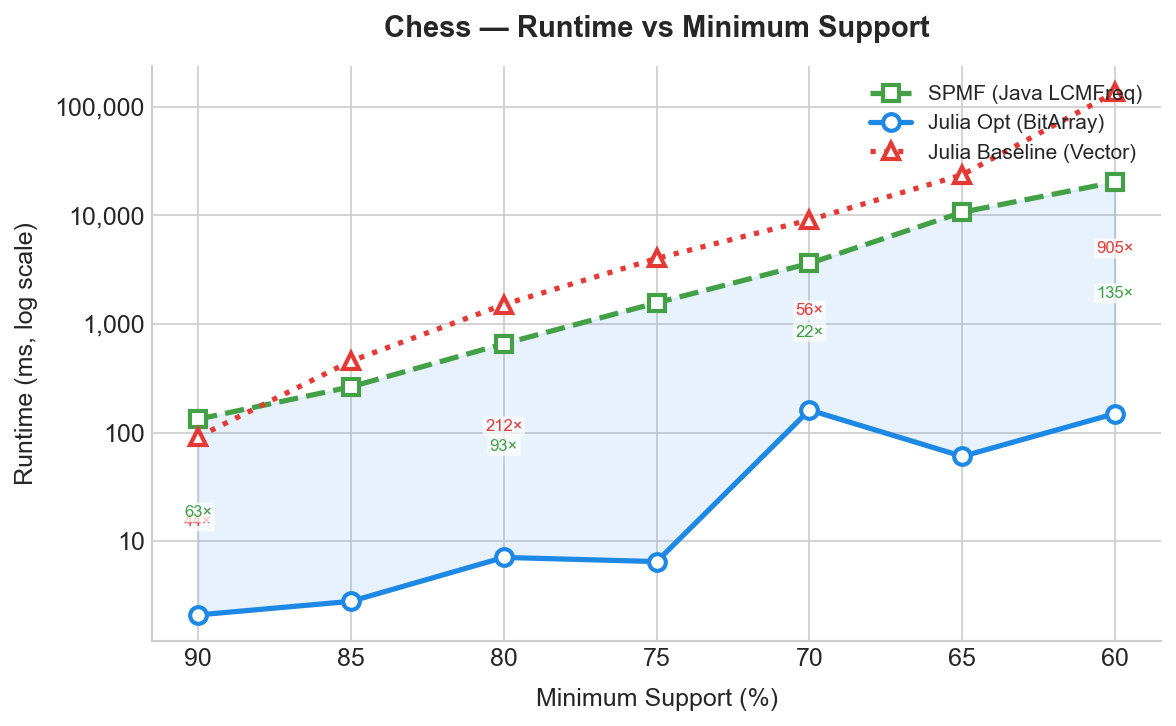
\includegraphics[width=\linewidth]{../data/results/figures/runtime_chess.png}
      \small Chess (dày đặc)
    \end{column}
    \begin{column}{0.48\textwidth}
      \centering
      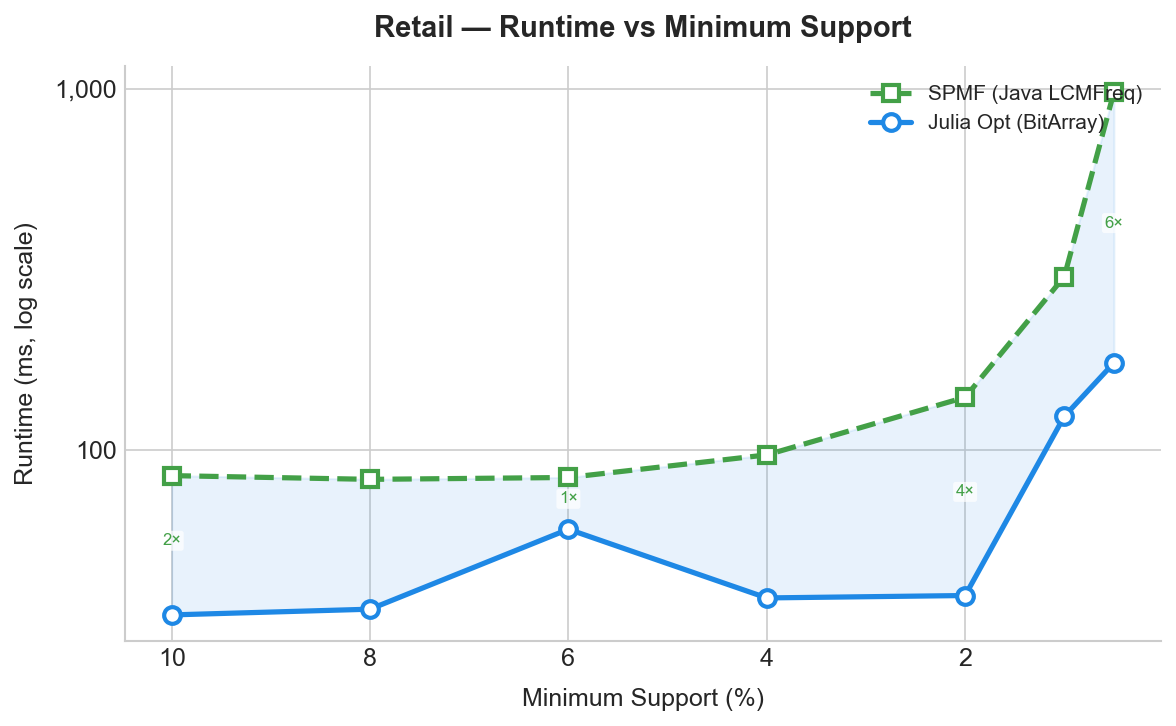
\includegraphics[width=\linewidth]{../data/results/figures/runtime_retail.png}
      \small Retail (thưa)
    \end{column}
  \end{columns}

  \vspace{0.2cm}
  \small
  Trục đứng là thời gian chạy theo thang logarithm. Trên dataset dày đặc
  như Chess, bản tối ưu nhanh hơn SPMF từ 76 đến 141 lần. Trên dataset thưa
  như Retail, mức tăng tốc khiêm tốn hơn (khoảng 2 đến 6 lần), vì denotation
  vốn đã nhỏ nên down project không tốn nhiều như trên dataset dày đặc.
  Baseline (vector số nguyên) hết bộ nhớ (OOM) trên Retail do cấp phát theo
  chỉ số item lớn nhất, trong khi Retail có tới 16\,470 item.
\end{frame}

% -------------------------------------------------------------------
\begin{frame}{Tăng tốc so với SPMF: tổng quan}
  \begin{columns}[T,onlytextwidth]
    \begin{column}{0.46\textwidth}
      \small
      \begin{tabular}{@{}lrrr@{}}
        \toprule
        Dataset & Trung vị & Min & Max \\
        \midrule
        Chess       & $135\times$ & $22\times$ & $241\times$ \\
        Mushroom    & $58\times$  & $23\times$ & $101\times$ \\
        Connect     & $6\times$   & $1\times$  & $34\times$ \\
        Pumsb       & $343\times$ & $12\times$ & $343\times$ \\
        Accidents   & $7\times$   & $2\times$  & $22\times$ \\
        Retail      & $2\times$   & $1\times$  & $6\times$ \\
        T10I4D100K  & $8\times$   & $4\times$  & $9\times$ \\
        T40I10D100K & $32\times$  & $21\times$ & $32\times$ \\
        \bottomrule
      \end{tabular}

      \vspace{0.15cm}
      \footnotesize Kosarak: SPMF không chạy được trên máy thực nghiệm, nên
      không có số liệu so sánh trực tiếp.
    \end{column}

    \begin{column}{0.50\textwidth}
      \centering
      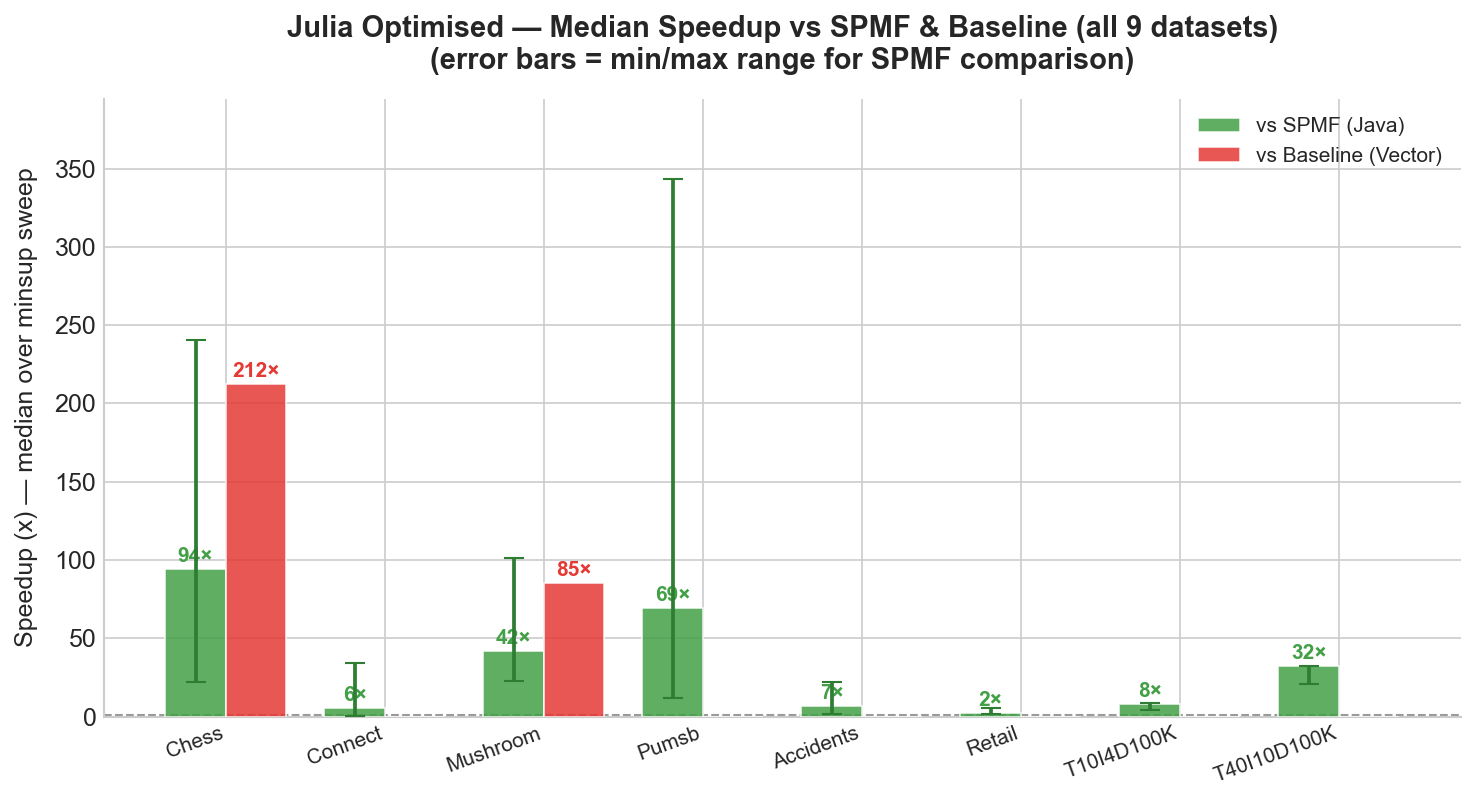
\includegraphics[width=\linewidth]{../data/results/figures/speedup_bar.png}
    \end{column}
  \end{columns}

  \vspace{0.15cm}
  \small
  Pumsb đạt mức tăng tốc cao nhất nhờ độ dài giao dịch trung bình lớn
  (74 item), khiến lợi thế của phép AND bit trên BitArray được khuếch đại.
\end{frame}

% -------------------------------------------------------------------
\begin{frame}{Số lượng frequent itemset theo minsup}
  \begin{columns}[T,onlytextwidth]
    \begin{column}{0.48\textwidth}
      \centering
      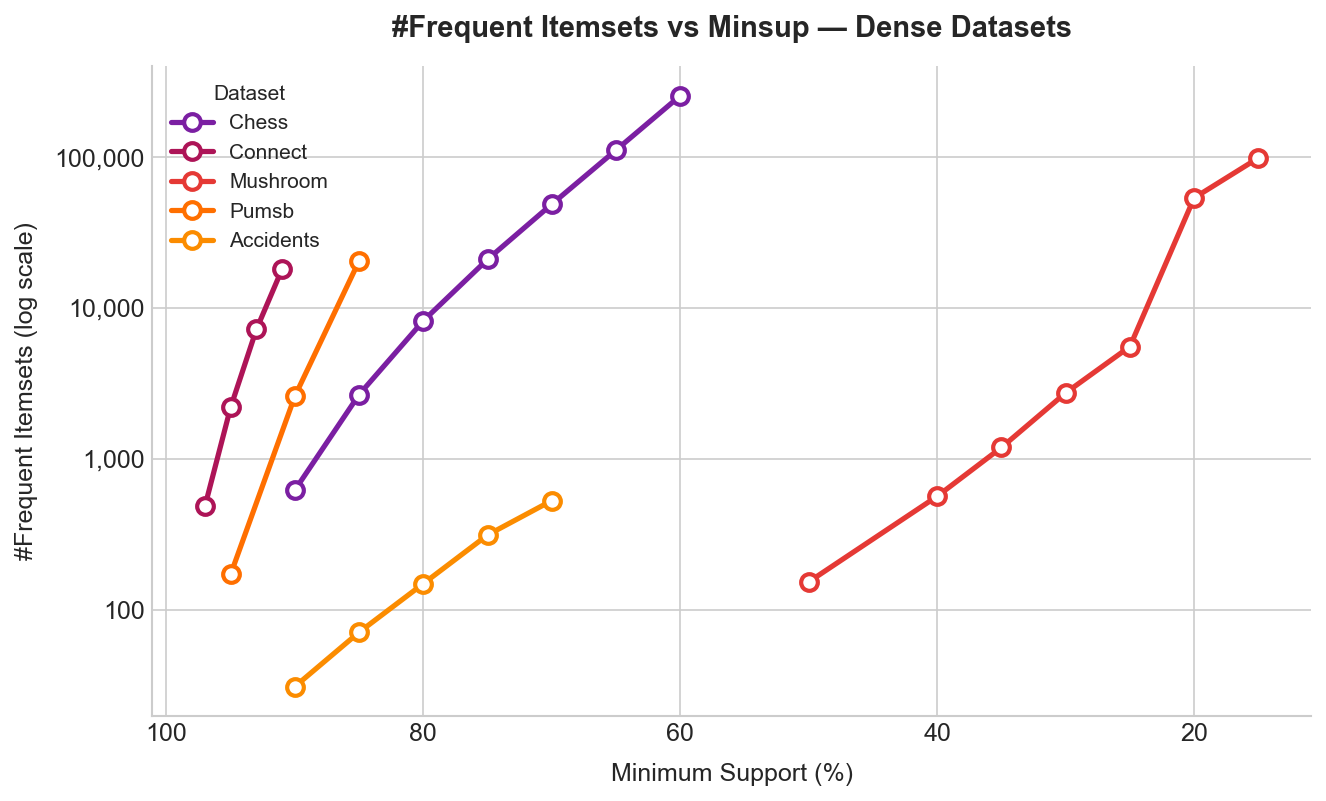
\includegraphics[width=\linewidth]{../data/results/figures/itemsets_dense.png}
      \small Dataset dày đặc
    \end{column}
    \begin{column}{0.48\textwidth}
      \centering
      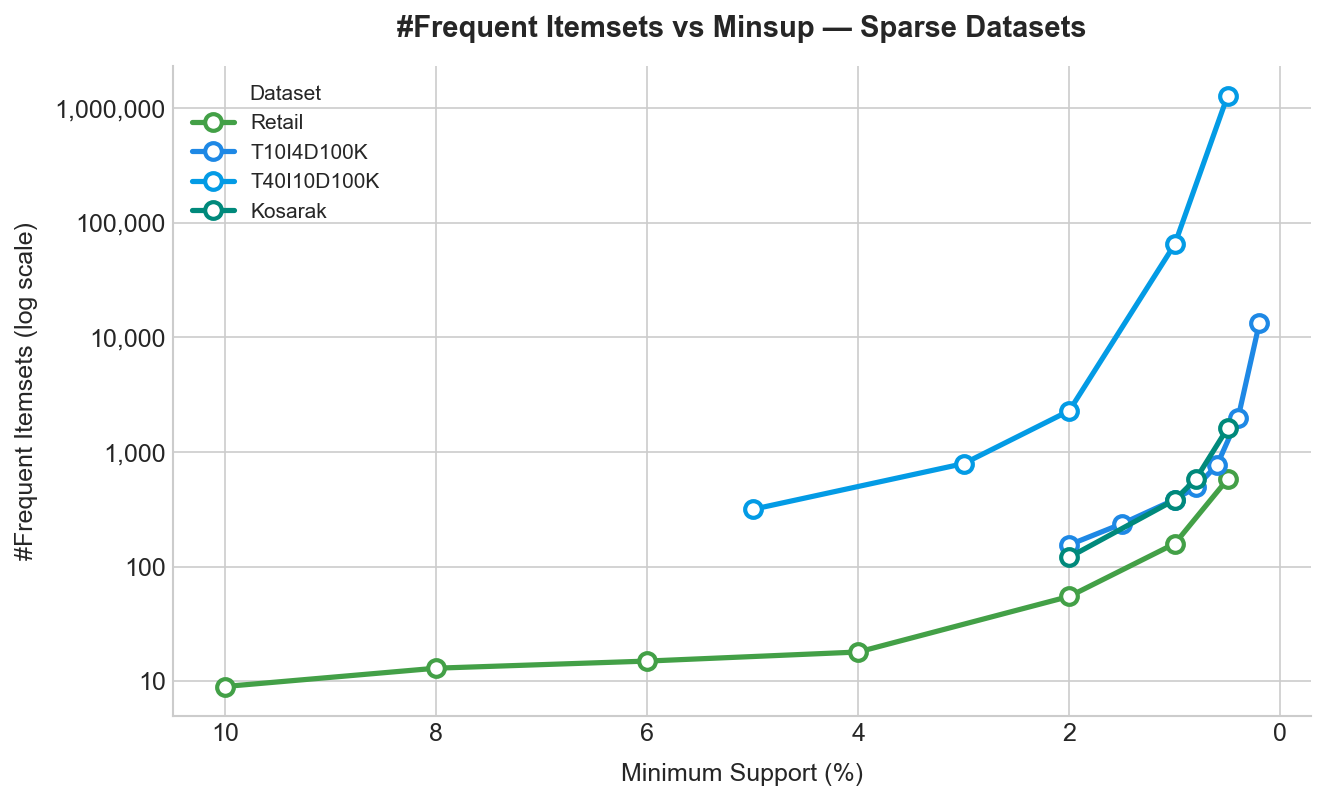
\includegraphics[width=\linewidth]{../data/results/figures/itemsets_sparse.png}
      \small Dataset thưa
    \end{column}
  \end{columns}

  \vspace{0.2cm}
  \small
  Khi $\sigma$ giảm, ngưỡng chấp nhận thấp hơn, cây tìm kiếm ít bị cắt tỉa
  hơn, nên số frequent itemset tăng theo dạng hàm mũ trên dataset dày đặc.
  Trên dataset thưa, số lượng itemset tăng chậm hơn nhiều, vì ít item đồng
  xuất hiện đủ thường xuyên để vượt ngưỡng. Đây là minh chứng thực nghiệm
  trực tiếp cho tính chất đơn điệu đã trình bày ở phần Đặt vấn đề.
\end{frame}

% -------------------------------------------------------------------
\begin{frame}{Sử dụng bộ nhớ}
  \begin{columns}[T,onlytextwidth]
    \begin{column}{0.42\textwidth}
      \small
      \begin{tabular}{@{}lrrr@{}}
        \toprule
        Dataset & Opt (MiB) & Baseline & Giảm \\
        \midrule
        Chess       & 31.87  & 857.23 & $26.9\times$ \\
        Mushroom    & 10.98  & 161.57 & $14.7\times$ \\
        Accidents   & 165.16 & OOM    & N/A \\
        Retail      & 20.68  & OOM    & N/A \\
        T10I4D100K  & 1\,215.2 & OOM  & N/A \\
        \bottomrule
      \end{tabular}
    \end{column}

    \begin{column}{0.54\textwidth}
      \centering
      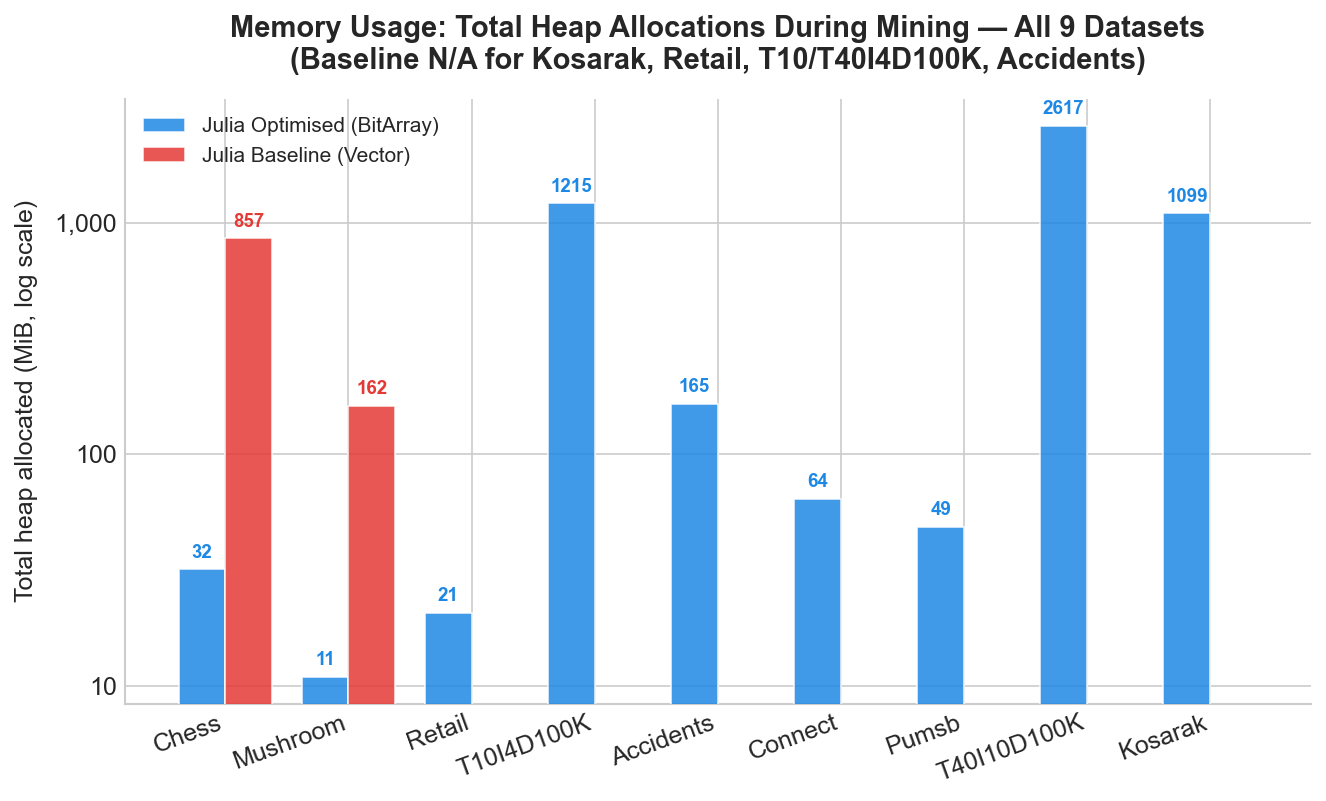
\includegraphics[width=0.98\linewidth]{../data/results/figures/memory.png}
    \end{column}
  \end{columns}

  \vspace{0.2cm}
  \small
  Baseline dùng \texttt{Vector\{Int\}} cho denotation, mỗi phần tử chiếm 8
  byte. BitArray chỉ chiếm 1 bit mỗi transaction, tiết kiệm khoảng $64\times$
  trên mỗi denotation. Baseline còn cấp phát mảng theo chỉ số item lớn
  nhất, gây lãng phí nghiêm trọng khi item ID thưa, ví dụ Retail có chỉ số
  item lớn nhất bằng 16\,470. Vì vậy baseline hết bộ nhớ trên 7 trong 9
  dataset. Bản tối ưu dùng cấu trúc kiểu từ điển, chỉ cấp phát cho item
  thực sự frequent, nên khắc phục hoàn toàn vấn đề này.
\end{frame}

% -------------------------------------------------------------------
\begin{frame}{Khả năng mở rộng theo kích thước dữ liệu}
  \begin{columns}[T,onlytextwidth]
    \begin{column}{0.46\textwidth}
      \small
      \begin{tabular}{@{}rrrr@{}}
        \toprule
        Tỉ lệ & Số transaction & Julia Opt (ms) & SPMF (ms) \\
        \midrule
        10\%  & 8\,816  & 9.0  & 57.0 \\
        25\%  & 22\,040 & 18.1 & 106.0 \\
        50\%  & 44\,081 & 22.9 & 157.0 \\
        75\%  & 66\,122 & 58.4 & 220.0 \\
        100\% & 88\,162 & 62.5 & 298.0 \\
        \bottomrule
      \end{tabular}

      \vspace{0.15cm}
      \footnotesize Lấy mẫu ngẫu nhiên không lặp từ Retail, minsup tuyệt
      đối tăng tỉ lệ với kích thước tập con, để giữ nguyên độ khó bài toán.
    \end{column}

    \begin{column}{0.50\textwidth}
      \centering
      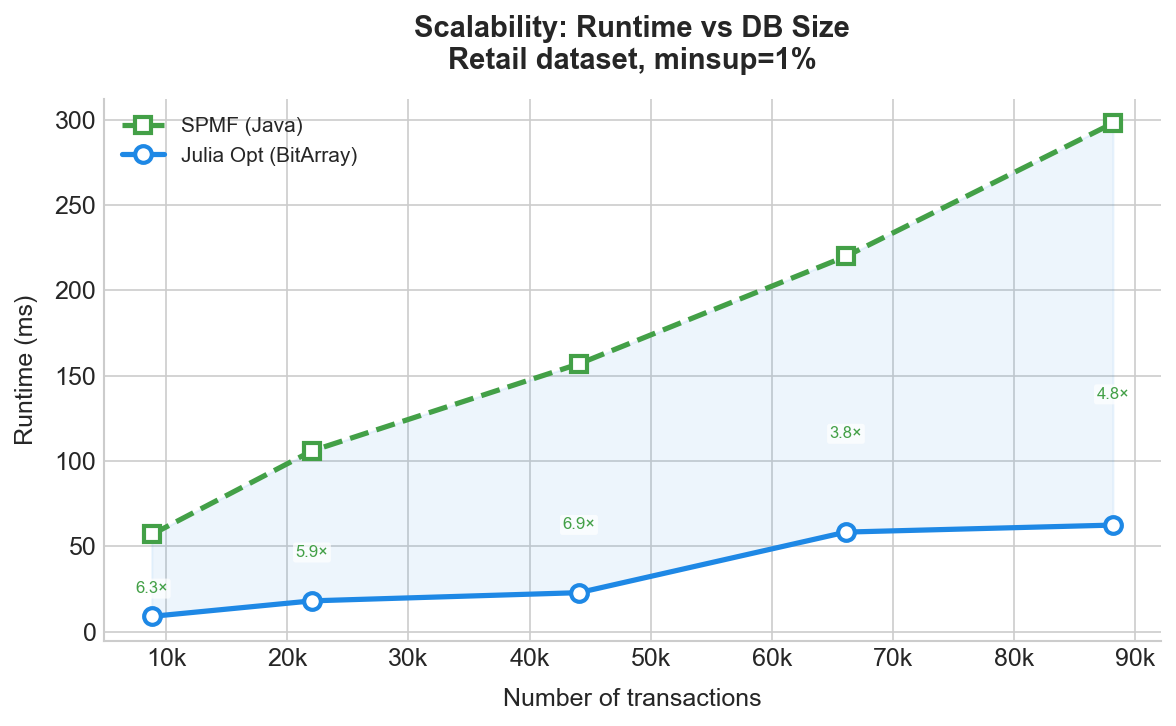
\includegraphics[width=0.96\linewidth]{../data/results/figures/scalability_by_ntx.png}
    \end{column}
  \end{columns}

  \vspace{0.15cm}
  \small
  Thời gian chạy tăng gần tuyến tính theo số transaction, đúng như lý
  thuyết: mỗi phép AND trên BitArray tốn thêm chi phí tỉ lệ với $n$ khi $n$
  tăng, còn số lượng itemset phổ biến giữ ổn định vì minsup tương đối
  không đổi.
\end{frame}

% -------------------------------------------------------------------
\begin{frame}{Ảnh hưởng của độ dài giao dịch}
  \begin{columns}[T,onlytextwidth]
    \begin{column}{0.48\textwidth}
      \centering
      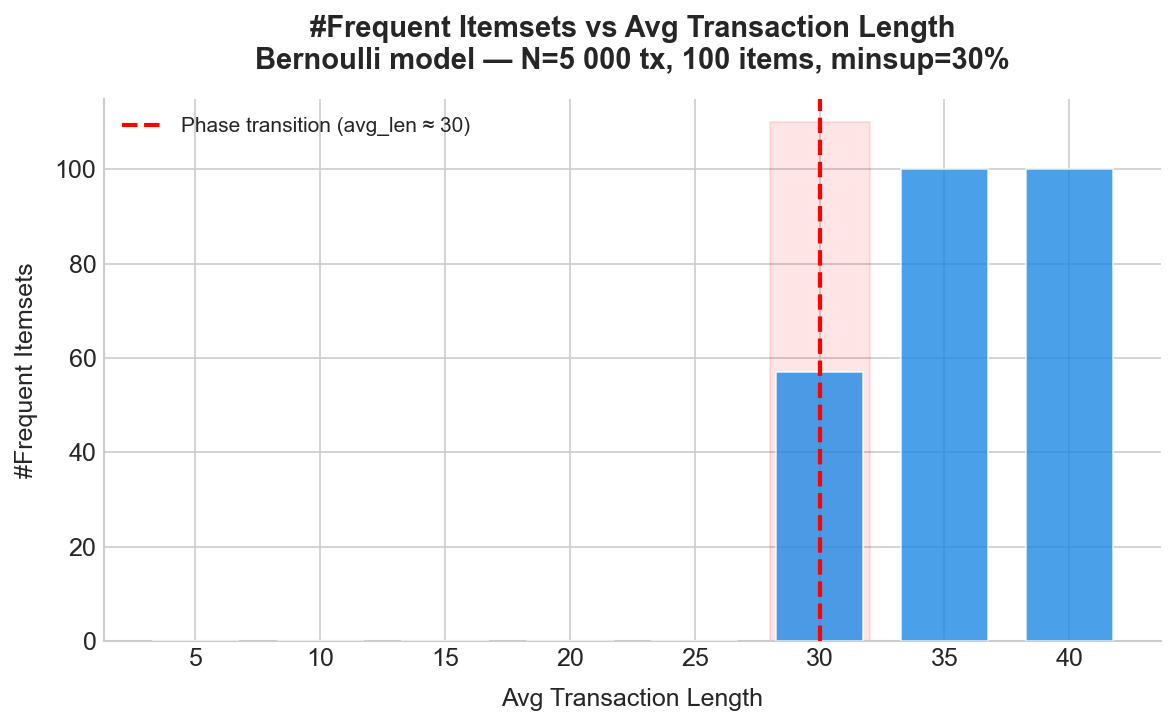
\includegraphics[width=\linewidth]{../data/results/figures/txlen_itemsets.png}
    \end{column}
    \begin{column}{0.48\textwidth}
      \centering
      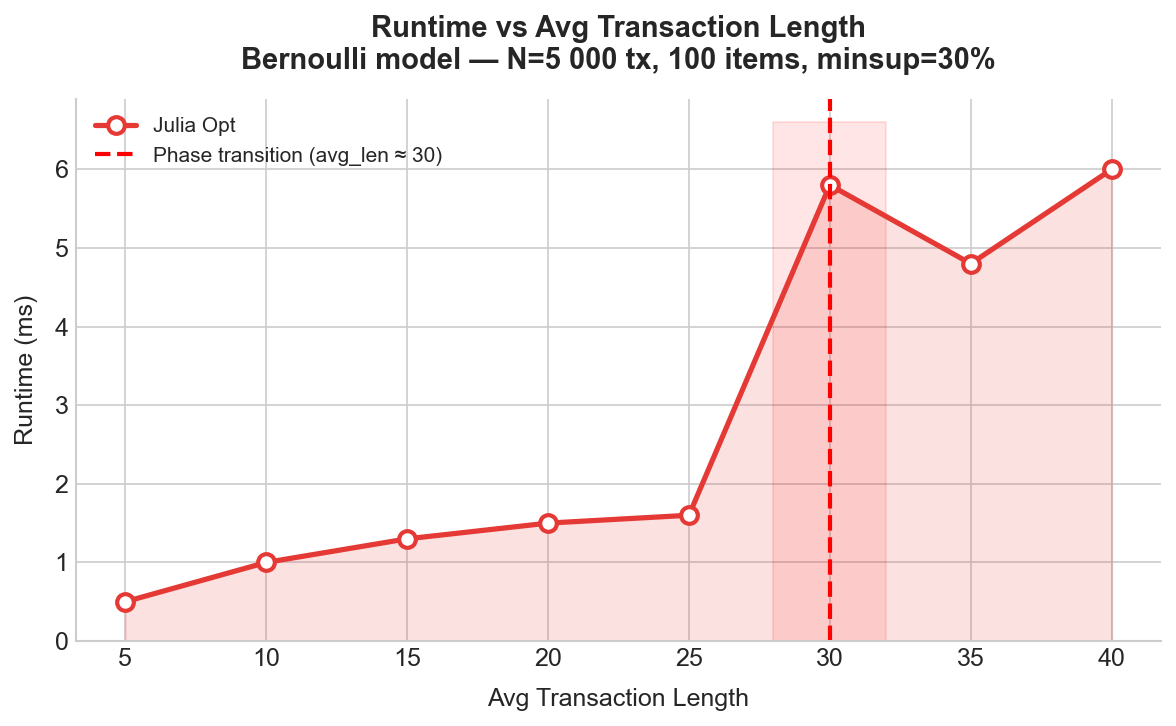
\includegraphics[width=\linewidth]{../data/results/figures/txlen_runtime.png}
    \end{column}
  \end{columns}

  \vspace{0.2cm}
  \small
  Dataset tổng hợp với 5\,000 giao dịch, 100 item, minsup $=30\%$ (ngưỡng
  tuyệt đối là 1\,500). Khi độ dài giao dịch trung bình nhỏ hơn 25, mỗi item
  chỉ xuất hiện trong khoảng 1\,250 giao dịch, chưa đủ ngưỡng, nên kết quả
  rỗng. Khi độ dài trung bình đạt khoảng 30, support kỳ vọng vượt ngưỡng và
  các itemset phổ biến bắt đầu xuất hiện đột ngột. Đây là ngưỡng pha
  chuyển (phase transition) của bài toán Frequent Itemset Mining.
\end{frame}

% ===================================================================
\section{Ứng dụng: phân tích giỏ hàng}
% ===================================================================
\begin{frame}{Sinh luật kết hợp từ kết quả LCMFreq}
  \begin{quietblock}{Từ frequent itemset đến association rule}
    Với mỗi itemset frequent $X$ và mỗi tập con khác rỗng $Y\subset X$, ta
    xét luật $Y\Rightarrow(X\setminus Y)$. Luật được giữ lại nếu độ tin cậy
    đạt ngưỡng tối thiểu:
    \[
      \mathrm{conf}(Y\Rightarrow X\setminus Y)=\frac{\mathrm{sup}(X)}{\mathrm{sup}(Y)}\geq\text{minconf}.
    \]
    Chỉ số lift cho biết mức tương quan so với việc hai vế độc lập:
    $\mathrm{lift}>1$ nghĩa là chúng có xu hướng đồng xuất hiện nhiều hơn
    ngẫu nhiên.
  \end{quietblock}

  \vspace{0.2cm}
  \small
  Thiết lập thực nghiệm trên dataset Retail (88\,162 giao dịch): minsup
  $=0.5\%$ ($\sigma=441$), thu được 580 frequent itemset; với minconf
  $=60\%$, sinh được 312 association rule.
\end{frame}

% -------------------------------------------------------------------
\begin{frame}{Top luật kết hợp theo lift trên Retail}
  \small
  \centering
  \begin{tabular}{@{}llrrr@{}}
    \toprule
    Vế trái & Vế phải & Support & Confidence & Lift \\
    \midrule
    $\{38,39\}$ & $\{41\}$     & 1.01\% & 0.89 & 8.7 \\
    $\{38\}$    & $\{39,41\}$  & 1.01\% & 0.82 & 8.1 \\
    $\{39,41\}$ & $\{38\}$     & 1.01\% & 0.80 & 7.9 \\
    $\{38,41\}$ & $\{39\}$     & 1.01\% & 0.78 & 7.7 \\
    $\{39\}$    & $\{38\}$     & 1.18\% & 0.73 & 7.2 \\
    $\{32\}$    & $\{48\}$     & 0.72\% & 0.78 & 6.4 \\
    \bottomrule
  \end{tabular}

  \vspace{0.25cm}
  \raggedright
  Nhóm sản phẩm $\{38,39,41\}$ có lift trên 7, cho thấy xác suất đồng xuất
  hiện cao gấp khoảng 7 lần so với ngẫu nhiên, là candidate mạnh cho chiến
  lược bán theo gói hoặc bố trí gần nhau trên kệ. Dataset Retail mã hóa sản
  phẩm bằng số nguyên, không có nhãn tên sản phẩm trong dữ liệu công khai,
  nên phân tích chỉ dừng ở mức item ID.
\end{frame}

% ===================================================================
\section{Kết luận}
% ===================================================================
\begin{frame}{Kết luận}
  \begin{columns}[T,onlytextwidth]
    \begin{column}{0.34\textwidth}
      \small
      \textbf{Đã hoàn thành}
      \begin{itemize}
        \item Cài đặt đầy đủ Backtracking, OccurrenceDeliver,
          HypercubeDecomposition theo đúng Uno et al. (2004).
        \item Bản tối ưu BitArray, kiểm thử đơn vị tự động.
        \item Khớp 100\% với SPMF trên toàn bộ 9 dataset.
        \item Ứng dụng phân tích giỏ hàng trên Retail.
      \end{itemize}
    \end{column}
    \begin{column}{0.32\textwidth}
      \small
      \textbf{Giới hạn}
      \begin{itemize}
        \item Bộ nhớ còn cao trên T10I4D100K (khoảng 1.2 GiB).
        \item Mỗi denotation vẫn lưu toàn bộ BitArray, chưa dùng diffset.
        \item Chưa khai thác đa luồng cho các nhánh DFS độc lập.
      \end{itemize}
    \end{column}
    \begin{column}{0.32\textwidth}
      \small
      \textbf{Hướng phát triển}
      \begin{itemize}
        \item Áp dụng diffset để giảm bộ nhớ khi support gần với node cha.
        \item Song song hóa các nhánh top level bằng đa luồng Julia.
        \item Mở rộng sang khai thác closed và maximal itemset (LCM gốc).
      \end{itemize}
    \end{column}
  \end{columns}

  \vspace{0.25cm}
  \begin{quietblock}{Tóm lại}
    LCMFreq dùng khung backtracking để tiết kiệm bộ nhớ so với Apriori, rồi
    khắc phục điểm yếu của backtracking trong việc đếm support bằng
    OccurrenceDeliver, và giảm số lần đếm lặp lại bằng HypercubeDecomposition.
    Bản baseline của nhóm bám sát mô tả của bài báo gốc, không dùng thư
    viện FIM có sẵn. Bản tối ưu giữ nguyên khung sinh itemset đó, chỉ thay
    cấu trúc denotation bằng BitArray để tăng tốc phép giao và đếm support,
    là đóng góp tối ưu hóa riêng của nhóm, không phải sao chép từ SPMF. SPMF
    chỉ được dùng làm chuẩn đối chiếu kết quả.
  \end{quietblock}
\end{frame}

% ===================================================================
\section{Tài liệu tham khảo}
% ===================================================================
\begin{frame}{Tài liệu tham khảo}
  \small
  \begin{enumerate}
    \item T. Uno, M. Kiyomi, H. Arimura. \textit{LCM ver.2: Efficient Mining
      Algorithms for Frequent/Closed/Maximal Itemsets}. IEEE ICDM Workshop on
      Frequent Itemset Mining Implementations (FIMI), Brighton, UK, 2004.
    \item R. Agrawal, R. Srikant. \textit{Fast Algorithms for Mining
      Association Rules}. Proc. 20th VLDB, pp. 487--499, Santiago, Chile, 1994.
    \item J. Han, J. Pei, Y. Yin. \textit{Mining Frequent Patterns without
      Candidate Generation}. Proc. ACM SIGMOD, pp. 1--12, Dallas, TX, 2000.
    \item M. J. Zaki, S. Parthasarathy, M. Ogihara, W. Li. \textit{New
      Algorithms for Fast Discovery of Association Rules}. Proc. 3rd KDD,
      pp. 283--286, Newport Beach, CA, 1997.
  \end{enumerate}
\end{frame}

\end{document}
